%%%%%%%%%%%%%%%%%%%%%%%%%%%%%%%%%%%%%%%%%%%%%%%%%%%%%%%%%%%%%%%%%%%%%%%%%%%%%%%%
%2345678901234567890123456789012345678901234567890123456789012345678901234567890
%        1         2         3         4         5         6         7         8

\documentclass[letterpaper, 10 pt, conference]{ieeeconf}  % Comment this line out if you need a4paper

%\documentclass[a4paper, 10pt, conference]{ieeeconf}      % Use this line for a4 paper

\IEEEoverridecommandlockouts                              % This command is only needed if 
                                                          % you want to use the \thanks command

\overrideIEEEmargins                                      % Needed to meet printer requirements.

% See the \addtolength command later in the file to balance the column lengths
% on the last page of the document

% The following packages can be found on http:\\www.ctan.org
\usepackage{graphics} % for pdf, bitmapped graphics files
\usepackage{epsfig} % for postscript graphics files
%\usepackage{mathptmx} % assumes new font selection scheme installed
%\usepackage{times} % assumes new font selection scheme installed
%\usepackage{amsmath} % assumes amsmath package installed
%\usepackage{amssymb}  % assumes amsmath package installed
\usepackage{subfig}
\usepackage{color}
\usepackage{url}

\graphicspath{{images/}}

\title{\LARGE \bf
Preparation of Papers for IEEE Sponsored Conferences \& Symposia*
}

\author{Akshaya Thippur$^{1}$, Rares Ambrus$^{1}$, Kaushik Desai$^{1}$, Adria Gallart$^{1}$, Malepati Sai Akhil$^{2}$, Gaurav Agrawal$^{2}$,\\Mayank Jha$^{2}$, Janardhan HR$^{2}$, Nishan Shetty$^{2}$, John Folkesson $^{1}$ and Patric Jensfelt$^{1}$% <-this % stops a space
\thanks{*This work was supported by STRANDS}% <-this % stops a space
\thanks{$^{1}$ KTH Royal Institute of Technology
        {\tt\small albert.author@papercept.net}}%
\thanks{$^{2}$ MSRIT Bangalore
        {\tt\small b.d.researcher@ieee.org}}%
}


\begin{document}

\maketitle
\thispagestyle{empty}
\pagestyle{empty}

%%%%%%%%%%%%%%%%%%%%%%%%%%%%%%%%%%%%%%%%%%%%%%%%%%%%%%%%%%%%%%%%%%%%%%%%%%%%%%%%
\begin{abstract}
\begin{quote}\
{\color{blue} AK: Not yet written, this is from the previous paper.}

Humans subconsciously exploit various strong correlations amidst different object instances, classes and between different object classes and scene types when analysing indoor environments. Correlations in naive, logical object co-occurrences have been exploited along with the extraction of vision based object-intrinsic descriptive features in previous research. In this paper, we present several alternative learning techniques to model and make estimates of scenes based on a variety of spatial relations - geometric extrinsic features with different amounts of discretization, which capture \textit{how} the objects co-occur; and compare their efficacy in the context of object classification in real-world table-top scenes. We investigate the possibilities of using such techniques to refine the results from a traditional vision-perception system. We also contribute a unique, long-term periodic, large 3D dataset of 20 office table-top scenes, manually annotated with 18 object classes. Apart from our current comparison, we foresee that the dataset will be useful for applications such as generalized learning of spatial models, learning object data structuring based on semantic hierarchy, learning best suited semantic abstractions and grammar for long term autonomy, ground truth for vision-perception systems etc.

\end{quote}
\end{abstract}

%%%%%%%%%%%%%%%%%%%%%%%%%%%%%%%%%%%%%%%%%%%%%%%%%%%%%%%%%%%%%%%%%%%%%%%%%%%%%%%%

\section{Introduction}
\label{sec:Introduction}

{\color{blue} AK: Needs shortening, has been modified from AAAI paper.}
{\color{red} PJ: Shorted and removed some things that are central to this paper. I think that the aim should be that this paper is cited not only for the dataset BUT also for showing, with hard data and not hand waving, that there are structures that can be exploited when building models and performing inference.}

In the last decades, computers have become part of human activities in all avenues of 
life and the field of intelligent autonomous robotics shows signs to follow in a 
similar way in the near future. In this paper, we concentrate our discussions on 
understanding and learning about indoor human environments, particularly office 
environments and suggestively toward understanding about human interactions with such 
environments.

% This fits better in the related work section. At least it has to move down because it comes too abruptly here
%
%Human environments are comprised of objects of various functionalities. It is crucial for 
%robots to learn the configuration of the objects and understand their utility if they are 
%to augment human activities. Cutting-edge object recognition, classification -- depend on 
%machine learning systems trained on intrinsic descriptive features extracted on the 
%objects present in the environment \cite{INCLUDE CITATION = Refer to a paper that actually is the source of such a statement, i.e. not the AAAI paper}. 
%Intrinsic feature based systems are susceptible to training noise, semantic noise and 
%systemic noise. More recently -- such systems also learn the statistics of co-occurrence 
%(extrinsic) of objects as additional features to gain robustness in performance.
%\cite{INCLUDE CITATION = AAAI paper}. The most recent aspect of object recognition based 
%scene classification and learning is to include the details of object co-occurrence in 
%terms of extrinsic geometrical features such as centroid distance vectors between 
%objects\cite{INCLUDE CITATION = Marina}, semantics based discretization of spatial 
%relations -- \textit{Next To}, \textit{In Front}, \textit{Left Of} etc. \cite{INCLUDE CITATION = relevant papers recently found}


% FROM AAAI -- State-of-the-art object recognition/classification typically relies on the extraction features to be matched against models built through machine learning techniques. As - the number of objects a given system is trained to recognise - increases, the uncertainty of individual recognition results tends to increase as greater number of objects increases the chance of overlapping features existence. The reliability of such recognisers is also affected when used on real robots in everyday environments, as objects may be partially occluded by scene clutter or only visible from certain angles, both potentially reducing the visibility of features for their trained models. In this paper we argue that the performance of a robot on an object recognition task can be increased by the addition of \emph{contextual knowledge} about the scene the objects are found in. In particular we demonstrate how models of the \emph{spatial configuration} of objects, learnt over prior observations of real scenes, can allow a robot to recognise the objects in unseen scenes more reliably. 

Our research work is performed in the context of developing a mobile service robot for long-term autonomy in indoor human environments, from 
offices to hospitals (Section~\ref{sec:Motivating Scenario}). 
The ability for a robot to run for weeks or months in its task environment opens up a new range of possibilities in terms of learning 
capabilities. In particular, the robot would expected to learn to perform an assigned task that is repetitive with weaning supervision and 
human interaction. The contextual knowledge the robot can gain from the repeated attempts can make it learn so that it's subsequent attempts 
on the same task are improved in accuracy and efficiency. 
In this paper we study \emph{table-top scene understanding} as a first step to such robotic behaviour. Whilst the objects present on a 
single table may change in position, their overall arrangement has some regularity over time as influenced by the context and functionality 
of the table-top. For example, there is a general structure in office employee table-tops to that of cafeteria table-tops or kitchen table-
tops. The differences derive from the variety of objects and their group-configurations on the table-tops with respect to time -- hours, 
days, weeks, months etc. For example: Office tables typically have monitors, keyboards, mouse along with papers and pens and coffee mugs 
configured such that the monitors can be viewed, the keyboard typed at and the mouse easily accessed from the keyboard. The spatial 
configuration vary in particular instances and the arrangement change gradually over many days and minutely at different times of the day; 
However, cafeteria tables have cutlery, jugs, food, napkins etc.\ configurations of which don't vary over many days, weeks or years but vary 
in content and presence according to different times of every day. It is this structure and it's variants that we aim to exploit in order to 
improve the understanding of table-top scenes.

Bluntly modelling the absolute positions of objects on tables, is likely to fail because such structure is improbable to 
generalise across a range of different types and instances of tables over numerous observations w.r.t.\ time. We are instead 
investigating qualitative \emph{relational} models of space, i.e. ways of encoding the qualitative position of a target object relative to 
the position of one or more landmark objects. For example: Given -- "A Keyboard is \textit{In Front} of a Monitor"; Depending on the size 
and span of the table and given knowledge about the functionalities and sizes of monitors and keyboards, humans can generally estimate a 
probable location for both objects on an unseen table. We believe that representations that are to support long term autonomy and ability to 
generalize knowledge require such rough discretizations of metric measurement space inherently encoding the generality of structure in the 
information. 

As a mean to study this, we have constructed a novel benchmark 3D data set of office type 
table-top scenes called \textit{\textbf{3D T}able-T\textbf{o}ps Dataset for Long \textbf{T}erm \textbf{A}utonomous \textbf{L}earning} (3D-
TOTAL)\footnote{\url{http://www.cas.kth.se/data/3D-TOTAL/}} observing the same set of select tables, over many times a day and over many 
days in a month. Objects-of-interest have been manually annotated in 3D to provide ground truth data. 

The main contributions of this paper are 3D-TOTAL dataset and the accompanying analysis that clearly show the potential presented by the 
structures that are inherent in the scenes for building models and for performing inference. 
The rest of the paper is structured in the following way: We survey the related work in Section~\ref{sec:Related Work} and present an 
example scenario for in Section~\ref{sec:Motivating Scenario}. In Section~\ref{sec:Dataset} we exhibit 3D-TOTAL in depth and provide an 
analysis of it in Section~\ref{sec:Analysis}. We summarize and conclude in Section~\ref{sec:Conclusions}.


% FROM AAAI -- (described in Section~\ref{sec:Dataset}), in this paper we explore the performance of a variety of representations for relative object position, plus inference techniques for operating on them, on the task of table-top scene understanding (Section \ref{sec:Techniques}). In particular we investigate representations that use varying forms of spatial relations, from geometric ones such as distances and angles to more qualitative spatial relations such as \textit{Left} and \textit{Behind} as a means for capturing observations of object configurations over time. The contributions this paper makes are: (1) A novel comparison between mechanisms for representing, learning and inference on object spatial configurations using spatial relations. (2) An evaluation of the use of these mechanisms for augmenting a robot's vision based \textit{perceptual system} (PS). (3) A new large 3D annotated table-top benchmark dataset.

%\subsubsection*{Points discussed}
%\begin{enumerate}
%	\item \textbf{Make this more "Human Oriented"}
%	\item Overview of the problem - why?
%	\begin{enumerate}
%		\item Not only desktops
%		\item How do we treat object classification
%	\end{enumerate}
%	\item Generalize and Transfer Knowledge
%	\item How are objects correlated, search becomes easier
%	\item Understanding a model for inter object influence for inference
%	\item No benchmarks yet or datasets having 3D spatial information
%	\begin{itemize}
%		\item time
%		\item complete scenes
%		\item different people
%		\item different types of people
%	\end{itemize}
%	\item need to structure data -- metric is tedious, because of large amounts of data
%	\item Contributions:
%	\begin{itemize}
%		\item A big 3D data set, annotated -- benchmark for results, folding data, classification.
%		\item suggest SR and QSR
%		\item something that could augment perception systems
%	\end{itemize}
%\end{enumerate}

%%%%%%%%%%%%%%%%%%%%%%%%%%%%%%%%%%%%%%%%%%%%%%%%%%%%%%%%%%%%%%%%%%%%%%%%%%%%%%%%

\section{Related Work}
\label{sec:Related Work}

{\color{blue} AK: Maybe needs shortening.}
{\color{red} PJ: Edited and shorted a bit.}

The dataset constructed in this work is motivated mainly by research pertaining to automatic learning about indoor human environments for 
long term autonomous robots. This requires certain characteristics of a dataset.

The \textit{B3DO dataset}~\cite{Janoch:ICCV2011} contains many single-snapshot instances of indoor human 
environments having a variety in viewpoints, object-classes, scene-classes and instances. This dataset is in the form of RGB and depth image 
pairs with manual 2D annotations of object classes. It captures single snapshots of unique scenes for which scene classification and object 
classification is difficult for vision based perception systems (VPS).
The \textit{NYU Depth V1-2}\cite{Silberman:ECCV2012} datasets contain different instance examples of object-classes and scene-classes 
captured with RGB+D images. Automated pixel clustering is conducted by using features in the RGB and D images separately and annotation of 
the clusters has been done manually, thereby assigning a semantic label to every pixel. The dataset contains a wide range of singular 
snapshots of indoor scenes from commercial and residential buildings. This dataset is primarily aimed at evaluating VPS aiming at automatic 
semantic segmentation and scene classification.

The \textit{3D IKEA database}~\cite{Swadzba:RAS2012} has been collected using a robot moving in different scene-class instances. The 
aim is to test scene-classification algorithms based on large, furniture level objects. 3D point clouds are formed by 
stitching a series of RGB+D images. There are very few small objects in the scenes and the annotations are provided at the 
scene-class level. The \textit{WRGBD dataset}~\cite{Lai:ICRA2011} is aimed to support object classification methods and contains many scene 
instances of isolated objects in point cloud format. Annotation is done by assigning every pixel a semantic label in each scene. Each point 
cloud is created from a series of RGB+D images.

The system constructed by~\cite{Russell:CVPR2009} can be used to automatically generate 3D datasets of scenes using rough human annotations 
on 2D images as input. The system infers 3D information from the scene using the semantics of the annotated properties of important planes 
in the image. The generated dataset thus includes a large set of singular scenes, indoor and outdoor from very particular viewpoints, with 
annotations to the image components provided manually.

The Kinect@Home project~\cite{Goransson13a} has collected a large set of crowd sourced data. People having access to a kinect like sensor 
have captured and uploaded data from their own environments. The data is in the form of RGB-D video sequences. The data covers a large 
variety of different scene types and range from single objects to whole rooms. No annotation is availble.

The dataset provided by~\cite{Sun:ECCV2010} contains a collection of 3D images of a few table-top objects in clear view and cluttered view. 
This dataset has been constructed to aid VPS for object classification and segmentation functioning on 3D data. Other datasets that have 
been developed have mainly been for training VPS for robust indoor object classification on 3D data~\cite{WillowGarage:2011,Kimmel:ACCV2010}.
However, none of these datasets contain the following three properties in their scenes:
\begin{itemize}
	\item complete 3D scene instances of a particular scene type (e.g.\ office table-tops, office rooms, cafeteria tables, hospital ward-
	rooms etc.)
	\item instances of subsets of objects-of-interest co-occurring in the scenes -- manually annotated for ground truth.
	\item long term periodic observations of the same set of scenes.
\end{itemize}
which are key for long-term autonomous scene model learning.

Scene learning and understanding can become a very expensive task if the raw data acquired by the 
sensors is used in terms of metric measurements. Many recent works have investigated how learning and modelling human 
environments increase in efficacy if qualitative spatial features are used instead of metric ones. Spatial relations have been used 
previously to provide contextual information to vision-related work;~\cite{MyungJin:CVPR2010} used a hierarchy of spatial relations 
alongside descriptive features to support multiple object detections in a single image. Spatial relations and contextual information are 
commonly used in activity recognition from video streams~\cite{Krishna:ECAI2010, Behera2012}. Recent work has used object co-occurrence to 
provide context in visual tasks such as activity recognition~\cite{Li:2012}. Apart from using the mere statistics of co-occurrence, a lot of 
information can be exploited from \textit{how} the objects co-occur in the scene. Recent work in 3D semantic labelling has used such 
geometric information along with descriptive intrinsic appearance features~\cite{Koppula:NIPS2011}. They achieve a high classification 
accuracy for a large set of object-classes belonging to home and office environments. Scene similarity measurement and classification based 
on contextual information is conducted by~\cite{Fisher:ACMT2011}. In~\cite{Aydemir:ICRA2011} spatial relations between smaller objects, 
furniture and locations is used for pruning in object search problems in human environments. In~\cite{Southey:2007,kasper:2011} the authors 
utilise both geometric features on objects and spatial relations between objects for scene understanding.

In our future work we aim to provide different representations of spatial context for a novel, long-term, learning task. Additionally the 
usage of such features leads to increased compatibility for robots to function using semi-supervised learning and in this way bootstrap the 
system using expert knowledge from humans.

%%%%%%%%%%%%%%%%%%%%%%%%%%%%%%%%%%%%%%%%%%%%%%%%%%%%%%%%%%%%%%%%%%%%%%%%%%%%%%%%

\section{Motivating Scenario}
\label{sec:Motivating Scenario}

{\color{blue} AK: I do not know if Patric wrote this part :-o.}
{\color{red} PJ: I did but it is not very grand in its current form}

We are investigating systems that operate for long periods of time in environments populated by humans. 
As a motivating scenario we will look at security guard in an office building. The robot patrols the working environment and should learn 
models of what the environment normally looks like and what variations there are. In an implementation of such a system the robot should be 
able to raise an alarm when something is not as expected. Initially we will focus on office table-top scenes. We are interested in models 
for individual desks and as well as general models of desks. Our working hypothesis is that there are some structures that govern how desks 
are organized. We want to extract and later exploit these when building the models. As mentioned above, we expect most desks to have a 
monitor, a keyboard and a mouse and that these are arranged in a certain way. Many people will have the mouse ot the right of the keyboard. This is an example of a spatial structure we want to learn. Some people have a laptop on their desk and they bring this 
laptop home in the evening. This is an example of a dynamic property of a desk that we want to learn.

Another aim is to be able to transfer knowledge from one desk to another and ultimately from one environment to to the next. That is, if the 
robot encounters a desk that it has not seen before, it should be able to make use of the models other desks to bootstrap the learning. This 
way, the robot would be able to perform some its functions even after a single observation, making it significantly more useful. The model 
of a newly observed desk would start out with relatively large uncertainty regarding what can be considered normal for that desk but this 
would improve over time as the model is adapted by new observations. To summarize, we strive to develop representations that caters for the 
knowledge transfer, the ability to learn from few samples and adapting existing models.

To study these questions we need data to learn from. The data need to capture both variations across different desks but also over time. 
None of the datasets available (see Section~/ref{sec:Related Work}) meet these requirements which is the motivation for the work behind the 
dataset that we present in this paper.

%\subsubsection*{Points Discussed}
%\begin{enumerate}
%	\item This section should stress why it is important to gather to such datasets
%	\item what type of data do we really need? - hint it
%	\item reference to related work section to show that this dataset is unique.
%\end{enumerate}

%%%%%%%%%%%%%%%%%%%%%%%%%%%%%%%%%%%%%%%%%%%%%%%%%%%%%%%%%%%%%%%%%%%%%%%%%%%%%%%%
\section{Dataset}
\label{sec:Dataset}


{\color{blue} AK: COMPLETED - needs refining.}

\begin{figure*}
\begin{center}
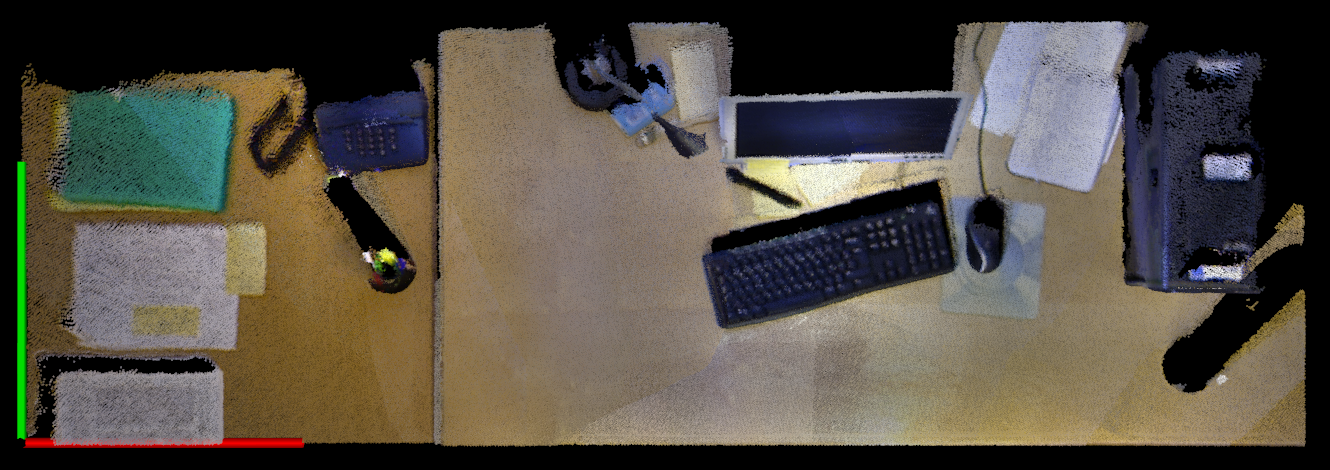
\includegraphics[height=2.5cm]{David_Mor_131110} \quad
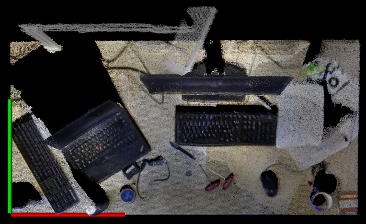
\includegraphics[height=2.5cm]{Nils_Mor_131111} \quad
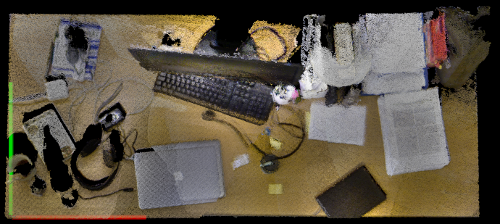
\includegraphics[height=2.5cm]{Puren_Eve_131029}\\ \smallskip
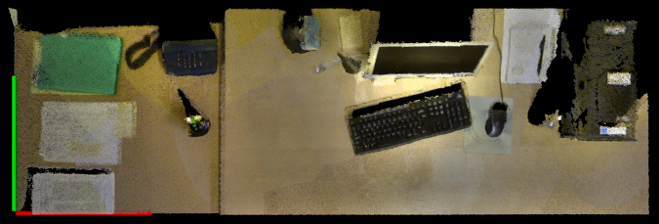
\includegraphics[height=2.5cm]{David_Eve_131110} \enskip
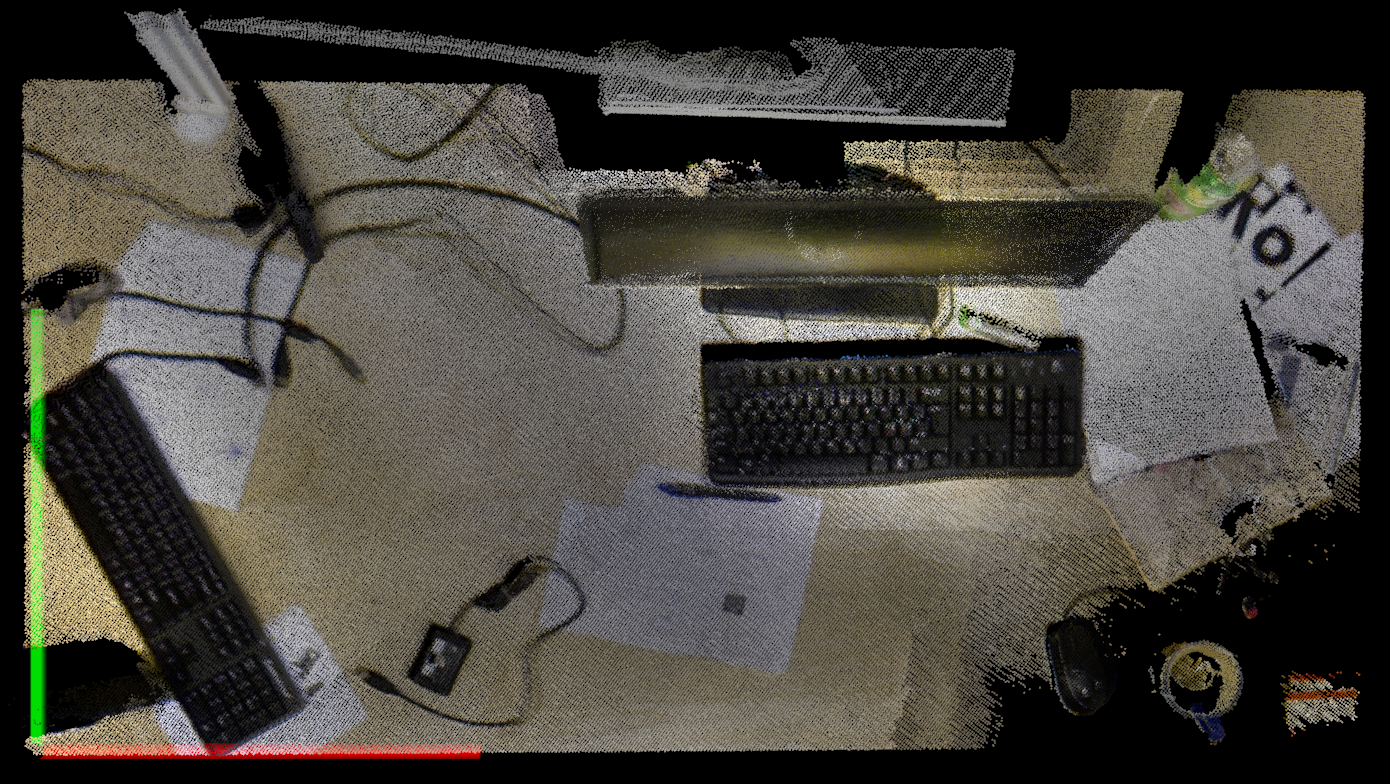
\includegraphics[height=2.5cm]{Nils_Eve_131111} \enskip
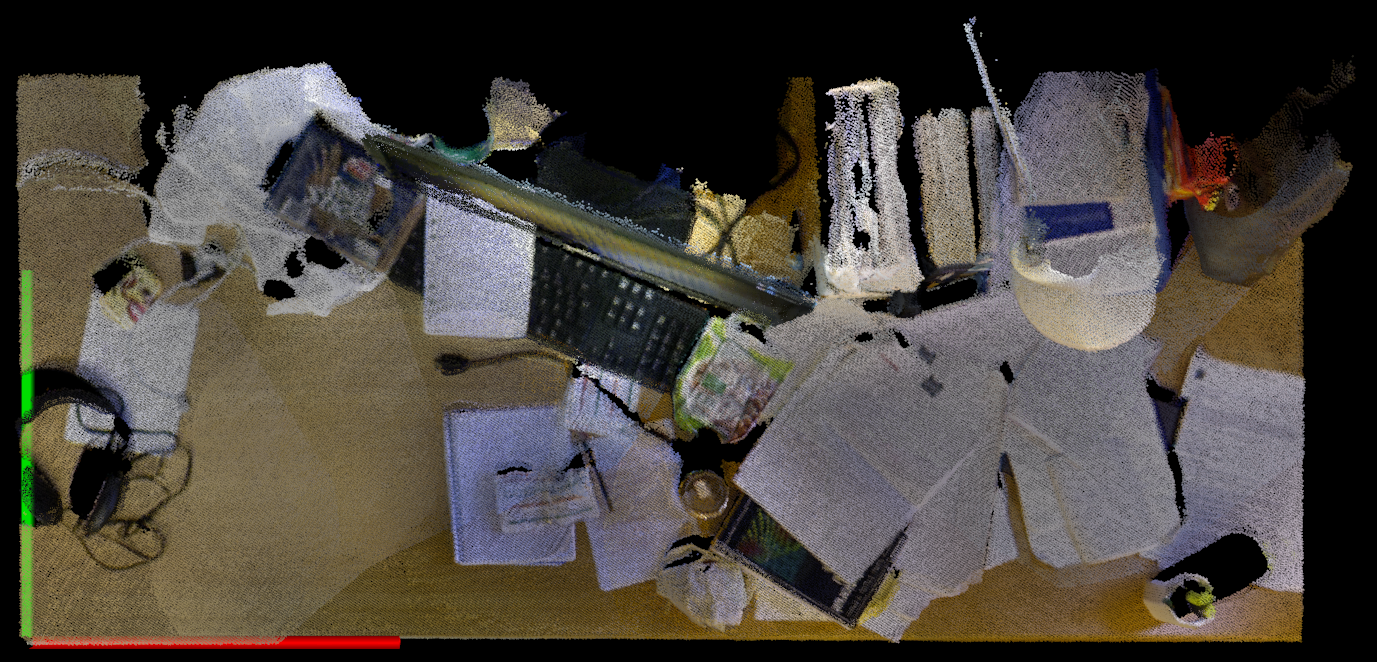
\includegraphics[height=2.5cm]{Puren_Mor_131110}
\caption{Each column shows a different person's office table in top view at two different times. The tables in the first two columns are captured in the morning and evening of the same day, whereas the table in the last column is captured 12 days apart. We can see distinct differences between different person's desk but there are also many commonalities that a system should exploit.}
\label{fig:Example Scenes}
\end{center}
\end{figure*}

Most of the human outdoor and especially indoor environments, are characterized by a supporting surface on which relevant objects are placed 
e.g. Land - buildings, living room floor - furniture, dining table - cutlery and dishes etc. It is hence convenient to perceive a structure 
for the object arrangement in the human environments to be as if on a "nested table-top system". Table-tops provide for a favourable 
prototypical example for analysis of object organization structure. 
% The below part is pushing in a direction which is not central to the paper and is reaching quite far without proper backup
%Moreover, it is highly likely that objects on a "table" have more semantic and organizational correlation amidst them, than when compared to those objects not on that same "table" e.g. \textit{Pen} has more semantic/functional correlation with a \textit{Laptop} (on the table) than a \textit{Couch} (not on that table, here the "table" references to the floor of the room).

With the aim of exploring possibilities to understand, learn and model these organizational structures amongst objects in human indoor 
environments, a first, pertinent dataset called 3D-TOTAL, has been composed by periodically capturing observations of a fixed set of entire 
table-tops in an office environment. In what follows we define a \textit{scene} as a single observation of a table-top instance at a single 
instance in time. The scenes have been captured as is\footnote{People have been asked to step aside not to contribute to the occlusion of 
the table-top.} with intervals of a few hours, over many days and populated with various instances of object classes. The dataset therefore 
captures the individual and group variation in object pose due to humans and their regular/irregular interaction with the environment. The required regularity in instances and time was the main motivation for the construction of this dataset, as currently available datasets either are of individual objects or single instances of tables or entire rooms. This regularity in sampling and extent over time is important when studying modeling interrelations amidst the member objects in a long-term autonomous learning. 

\subsection{Dataset Design and Concept}
\label{ssec:Dataset Design and Concept}
%\subsubsection*{Points Discussed}
%\begin{enumerate}
%	\item Why did we collect it the way we did?
%	\item What did we collect?
%	\item Time and people level slicings
%	\item weekends and weekdays
%	\item different times of the day
%	\item We want the data to have these properties and hence we designed the dataset in this way.
%\end{enumerate}
%The target research groups to benefit from this dataset are of the kind that develops artificial intelligence for autonomous robots 
%augmenting human activities (especially if they are fatiguing) within indoor human environments. Hence, it becomes essential for robotic 
%learning to pay attention to variances in human environments wrt. scales of time, space and instances in the same space. 
As explained in Section~\ref{sec:Motivating Scenario} our research intentions are to provide intelligence to an long-term operating, 
autonomous robot for indoor human environments. Thus, the concept of composing the 3D-TOTAL dataset follows naturally from this research 
motivation. The dataset has been composed by capturing and manually annotating 3D point clouds of office type table-tops, for a fixed set of 
people, at fixed times of the 
day and for a span of weeks. Observing the table-tops of the same set of people at different times of the day gives insight about the daily 
interactions a human has with his table and over many days gives an understanding of the gradual variances of their table-tops. If the data 
is observed for an entire week, including weekends, features in the table-top configurations, that can be used for estimation of the type of 
the day of the week, can be extracted (e.g.\ Weekdays, Fridays, Weekends). Table-top models can also be learnt for all the people put 
together -- which gives a gross functional representation of an office table-top in general in office environments -- or for individual 
people which helps to build functional representations of office table-tops for individuals, for different activities and so on 
(Figure~\ref{fig:Example Scenes}). 
%Finally, when trying to find general models over any of these types of data partitions, the model learns 
%to be able to generalize over different instances of a fixed set of object classes. 
In summary: When the dataset is partitioned in different ways with respect to time, people or object instances, it richly yields knowledge 
of table-tops in office environments supporting building representations of the same.

\subsection{Dataset Realization}
\label{ssec:Dataset Realization}
%\subsubsection*{Points Discussed}
%\begin{enumerate}
%	\item Annotation Tool
%	\item Tools for collecting Asus Scenect
%	\item 
%\end{enumerate}
In 3D-TOTAL, 3D point clouds representing 20 people's desks were captured regularly 3 times a day for 19 days. The data was collected by 
carefully scanning each table-top using an \textit{Asus Xtion Pro Live} RGB-D camera. The raw RGB-D data stream is aggregated into a single 
high resolution point cloud (.pcd format) using the \textit{SCENECT} software~\cite{Buerkler:Online2012}.

The scenes were recorded as periodically as possible and at three fixed times each day: \emph{Morning} (09:00 hrs), \emph{Afternoon} (13:00 
hrs) and \emph{Evening} (18:00 hrs). Scenes contain tables of 20 different people collected over 19 days including weekends. 
A \textit{Scene\_ID} is attached to each scene to indicate who the table belongs to and the date and time of the recording. These Scene\_IDs help in partitioning the dataset with respect to time of the day \{Morning, Afternoon, Evening\}, person \{Carl, Nils, \dots\}, or day \{2013-11-01, 2013-11-06, 2013-11-13, \dots\}.

A 3D annotation tool was developed for manually segmenting out objects-of-interest from the point clouds. On average, 12 different objects 
were labelled, including repeating instances of the same object class, per scene depending upon feasibility and occurrence. The objects 
belong to the following super set - \{Mouse, Keyboard, Monitor, Laptop, Cellphone, Keys, Headphones, Telephone, Pencil, Eraser, Notebook, 
Papers,  Book, Pen, Highlighter, Marker, Folder, Pen-Stand, Lamp, Mug, Flask, Glass, Jug, Bottle\}. The information about every scene and 
object is available in  XML and JSON formats. Each scene has a nested list of object data containing \{Position, Orientation, Size, Date and 
Time of recording, Person ID, Point Indices of the points in the point cloud that have been labelled as belonging to the Object\}. This 
manual annotation provides the required ground truth data for long term autonomous learning.

\subsection{Dataset Summary}
\label{ssec:Dataset Summary}
This section gives a brief summary of the dataset to serve as a quick reference.
\noindent 3D-TOTAL has:
\begin{itemize}
	\item scenes collected from 20 unique tables, 3 times a day for 19 days and hence in total, approximately 1140 scenes.
	\item each scene manually annotated with 18 possible object classes and an average of 12 object instances, from these classes, annotated per scene.
	\item has annotation stored in XML and JSON formats containing scene instance and it's object instances' specifications.
	\item occurrences of object instances as depicted in Figure~\ref{fig:HistOfObjects} and annotations as exemplified in Figure~\ref{fig:RawPCD},\ref{fig:RawPCDAnnotated}
\end{itemize}

\begin{figure}[t]
\begin{center}
\subfloat[][]{\label{fig:HistOfObjects}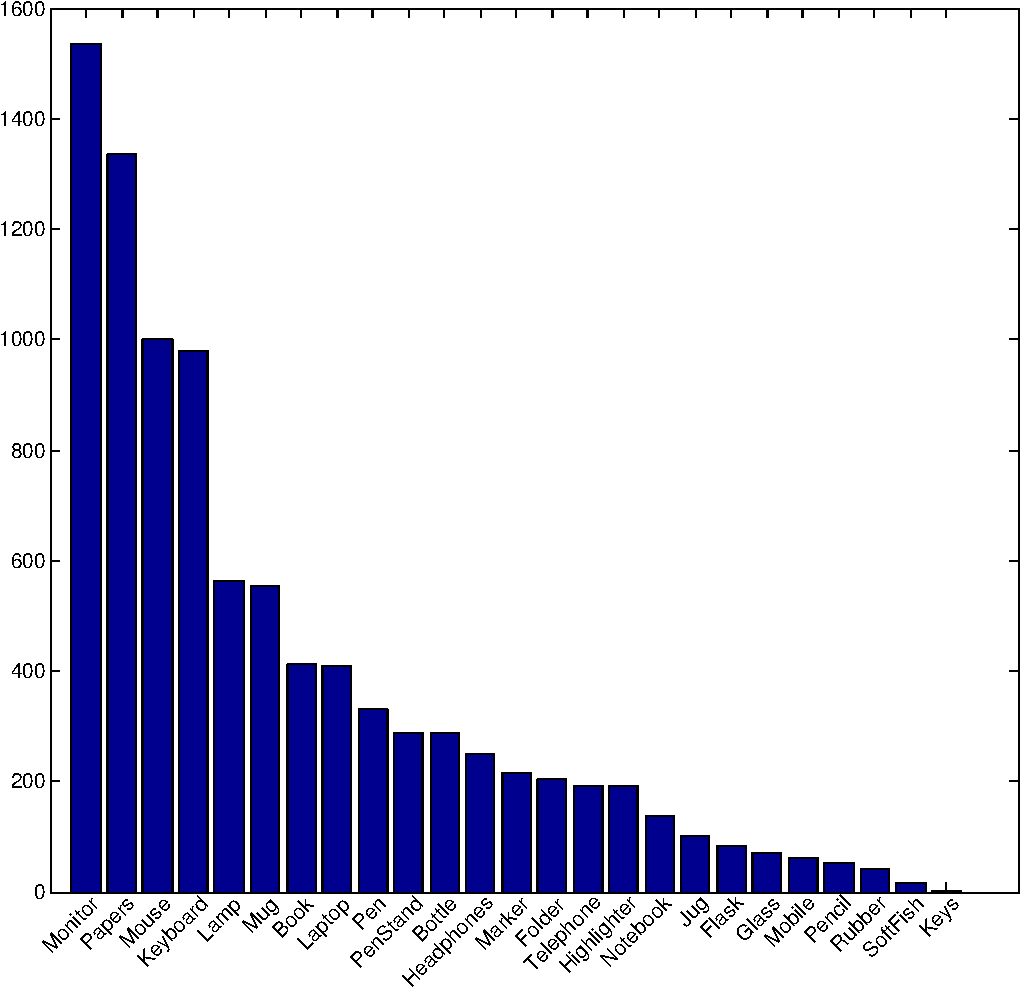
\includegraphics[width=0.8\linewidth]{HistOfObjects_crp.pdf}}\\
\subfloat[][]{\label{fig:RawPCD}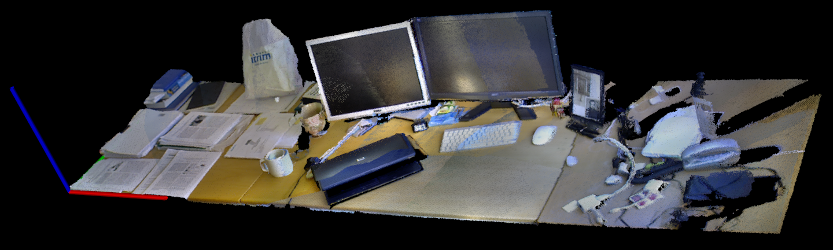
\includegraphics[width=0.7\linewidth]{pcd.png}}\\
\subfloat[][]{\label{fig:RawPCDAnnotated}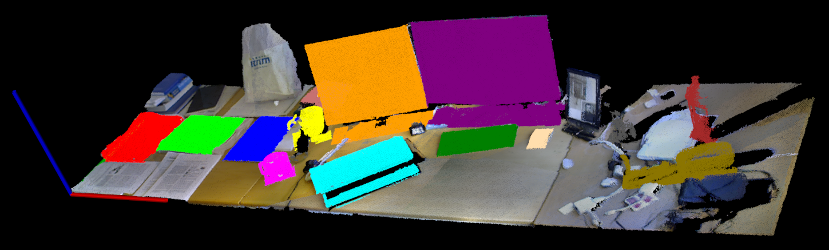
\includegraphics[width=0.7\linewidth]{pcd_annotated.png}}
\caption{(a) Objects annotated in 3D Long-Term Dataset, sorted in descending order of count of occurrences. X-axis$=$Object Name, Y-axis$=$Occurrence Count. (b) Screenshot of one table scene, along with it's annotations in (c).}
\end{center}
\end{figure}

%%%%%%%%%%%%%%%%%%%%%%%%%%%%%%%%%%%%%%%%%%%%%%%%%%%%%%%%%%%%%%%%%%%%%%%%%%%%%%%%

\section{Analysis}
\label{sec:Analysis}


{\color{blue} AK: Patric wrote this part, I am yet to look at it.}

In this section we perform an analysis of the data to highlight some interesting aspects of it. In particular we want to show that 
there are structures in the data that can be exploited by a system for more efficient representations and better reasoning with less data.

Figure ~\ref{fig:Example Scenes} shows three desktop scenes. Each column shows the same desk at two different times. The leftmost two columns 
contain scenes from the same day, whereas the two scenes in the third column were sampled 12 days apart in time. Notice in Column 1: the slight changes in 
position of the keyboard, mouse, papers and pen; Column 2: the relatively big changes in position of laptop, mouse, papers, pen, keyboard, 
lamp. When objects in columns 1,2,3 are compared there is a certain generality in structure (keyboards are in front of monitors), but 
also a specificity for each person (occurrence of headphones, position of mouse w.r.t.\ keyboard, etc.). Studying the scenes could also allow a system to 
infer the activity of people. We can see that there are changes to the first desk suggesting that someone 
was there during the day and that this person is quite well-ordered. The second table misses the laptop in the second observation. This might suggest that 
the person has left the desk, maybe for the day. The third desk seems to be occupied by someone that is less sensitive to 
clutter. With only two observations of each desks these are just speculations but by looking at the data over 19 days stronger claims coud be made.

One of our hypotheses is that a qualitative model will be needed to achieve efficient and powerful representations of 
space, at least if the amount of data is limited as it will be in realistic cases. Such qualitative models could allow some of the inherent 
structure in the environment be encoded in the representation itself. We have already seen in Figure~\ref{fig:Example Scenes} that monitors 
are typically in the back while a keyboard is usually in front of it and the leftmost table shows an example of a mouse being to the right of a keyboard. Figure~\ref{fig:scatter-keyboard-mouse} shows a scatter plot 
over the position of keyboards and mice when found in the same scene. The table outline gives an example of a prototypical desk to make it easier to interpret the data. 
In the top part of the figure, the green circles mark the position of the centroid of each 
keyboard that exist in a scene where there is at least one mouse. The red square shows the mean position of all these centroids. The black 
crosses show the position of all mice in scenes with at least one keyboard. In the bottom part of the figure the position of the mouse 
relative to the keyboard is shown for each observed pair in the data. As expected most mice are qualitatively to the right of the keyboard. There are some outliers. However,  
encoding the position of the mouse as being to the right of a keyboard would capture most of the information. The largest cluster of points in the lower part of Figure~\ref{fig:scatter-keyboard-mouse} contains 95\% (CHECK THIS!!!!) of all data points. Notice how this structure in the data is lost, at least visually, when looking at the position of the keyboard and mouse in the table frame (top figure) and how it pops out when looking at the relative positions (bottom figure). We want our representation to be able to capitalize of this structure. Clearly, in this case, the position of the keyboard contains almost all information that is needed to represent the position of the mouse as well.

\begin{figure}
\begin{center}
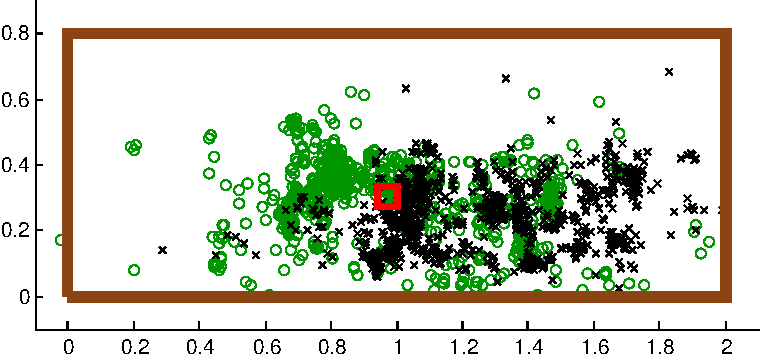
\includegraphics[width=0.8\linewidth]{keyboard_mouse_raw-crop}
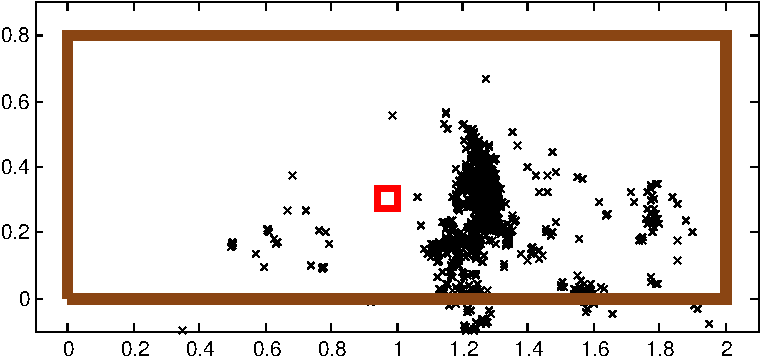
\includegraphics[width=0.8\linewidth]{keyboard_mouse-crop}
\end{center}
\caption{Top: The green circles shows the positions keyboards(red square shows mean of keyboards). The black crosses show the position of all mice in these scenes. Bottom: Mean position of keyboards (red square) and relative position of mouse relative to it. The brown rectangle gives a rough idea about where the borders of a typical desk would be.} 
\label{fig:scatter-keyboard-mouse}
\end{figure}

To further investigate the correlation between different object classes, and thus look for other inherent structures in the data, we look at 
the relative position of all objects of class $C_j$ w.r.t.\ to objects of class $C_i$ present in the same scene. To get a quick 
overview of the type of distributions this results in we look at the entropy of these distributions. A large entropy (closer to uniform 
distribution) would suggest that the objects are largely uncorrelated and a small entropy (a more peaky distribution) a stronger 
correlation between the objects. We calculate the entropy as 
\begin{equation}
E=-\sum (\frac{n_i}{N})ln(\frac{n_i}{N})
\end{equation}
where $n_i$ is the number of samples that fall in cell $i$ in a grid discretization of the table and N is the total number of samples. Each 
sample correspond to one object pair in one scene. The true entropy will only be estimated well when $N$ is large. We therefore limit this 
investigation to pairs of objects that occur more than a certain number of times in the data. Figure~\ref{fig:entropy} shows these entropies 
for 10 of the objects in the dataset. From this figure we can, for example, see the low entropy in the relation between keyboard and mouse (
element 1,3 and 3,1 in the matrix). The relative positions of monitors and keyboards also have a fairly low entropy. We also see that the 
position of papers is largely uncorrelated with many other objects (uniform distribution gives high entropy). 

In Figure~\ref{fig:scatter-rest} we look closer at some of these relations. Figure~\ref{fig:scatter-monitor-keyboard} shows the position of 
the keyboard w.r.t.\ to the monitors. Our intuition that keyboards are placed mostly in front of monitors is supported by data. 
Figure~\ref{fig:scatter-keyboard-mug} shows the position of the mug w.r.t\ the keyboard. We see that the mug is rarely very close to the center of the 
keyboard but rather positioned around the keyboard. Taking function into account the data might suggest that the mug 
is in fact often placed at arms length from the person working on the desk to keep it at safe distance from the keyboard but still within 
reach. We see a bias towards the right side, probably a result of most people being right-handed. In Figure~\ref{fig:scatter-keyboard-papers} we see 
that the distribution for the relative position of papers w.r.t.\ to the keyboard is almost uniform, suggesting that they are largely uncorrelated. The fact that there are often many papers in a scene adds to the uniformity.

\begin{figure}
\begin{center}
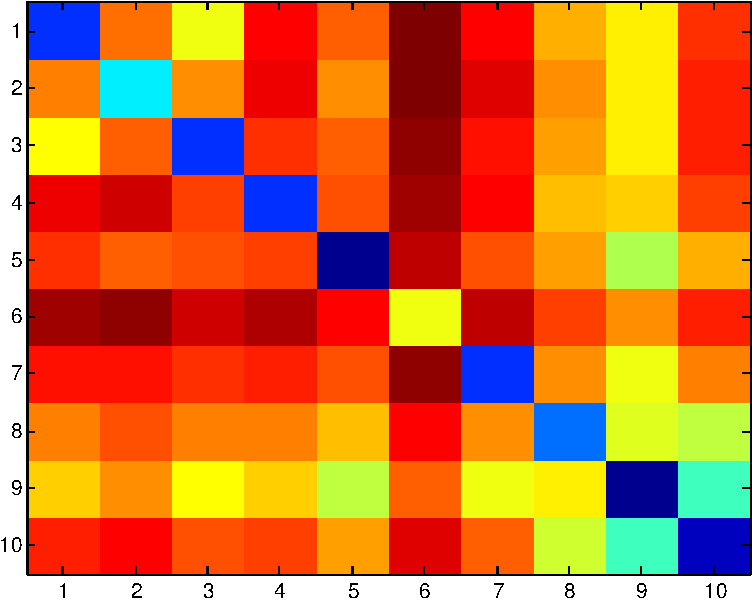
\includegraphics[width=\linewidth]{entropy_matrix-crop}
\end{center}
\caption{The figure illustrates the entropy in the distribution of relative positions of one objects (column) w.r.t. to another objects (row). Dark red indicates high entropy (more uniform distr.) and dark blue low entropy (peakier distr.). We show this for a subset of objects from the database; 1:keyboard, 2:monitor, 3:mouse, 4:mug, 5:laptop, 6:papers, 7:book, 8:bottle, 9:jug, 10:notebook. }
\label{fig:entropy}
\end{figure}

%\begin{itemize}	
%\item keyboard
%\item monitor
%\item mouse
%\item mug
%\item laptop
%\item papers
%\item book
%\item bottle
%\item jug
%\item notebook
%\item mobile
%\item glass
%\item flask
%\end{itemize}

\begin{figure}
\begin{center}
\subfloat[][]{\label{fig:scatter-monitor-keyboard}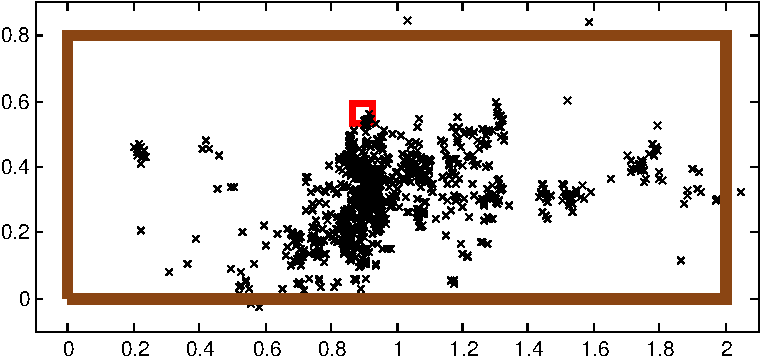
\includegraphics[width=0.8\linewidth]{monitor_keyboard-crop}}\quad
\subfloat[][]{\label{fig:scatter-keyboard-mug}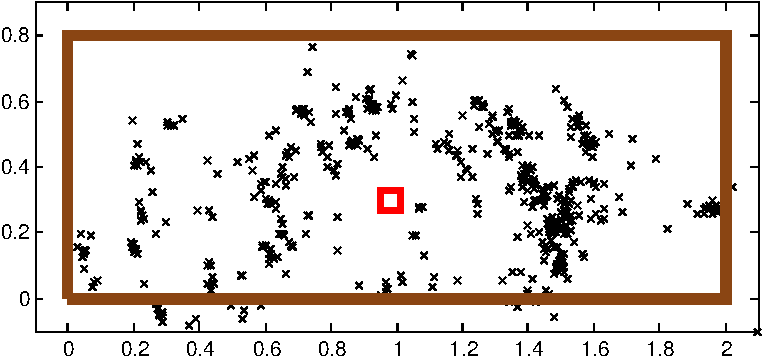
\includegraphics[width=0.8\linewidth]{keyboard_mug-crop}}\\
\subfloat[][]{\label{fig:scatter-keyboard-papers}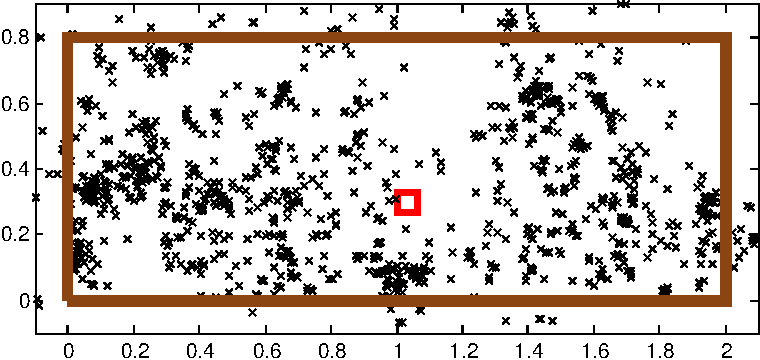
\includegraphics[width=0.8\linewidth]{keyboard_papers-crop}}
\end{center}
\caption{The figures show the relative position of a) keyboard w.r.t. monitor, b) mug w.r.t. keyboard and c) papers w.r.t. keyboard. Qualitatively keyboards are mostly infront of monitors, mugs are around the keyboard and the position of papers is mostly independent on the position of the keyboard.} 
\label{fig:scatter-rest}
\end{figure}

To summarize the analysis, we have shown that the data has many structural properties that a method for representing and reasoning about 
space should exploit. If the aim is to represent typical configuration of objects, this preliminary analysis suggests that a significant 
part of such knowledge can be encoded well with qualitative spatial relations, such as the mouse is to the right of the keyboard, while 
keeping in mind that this represents the typical case and not the only possible situation. We can also see that a system that observes these desks for 
an extended period of time will be able to learn quite a lot about the habits of the owners of the desks and even the current activity in 
many cases. It is important to differentiate between typical knowledge, i.e., knowledge about what the world typically is like and specific 
instance knowledge, i.e., knowledge about a particular scene at a specific time. It is to capture the first kind of knowledge that we 
believe  qualitative spatial representations will be most beneficial. 

%\subsubsection*{Points Discussed}
%\begin{enumerate}
%	\item \textbf{figure} Scatter plot for variation within person ID
%	\item \textbf{figure} Scatter plot for variation wrt object type
%	\item \textbf{figure} Scatter plot for variation considering different landmark - trajectors.
%	\item \textbf{figure} Scatter plot of 2D footprints of objects
%	\item General conclusions about above figures.
%	\item 
%	\item 
%\end{enumerate}

%%%%%%%%%%%%%%%%%%%%%%%%%%%%%%%%%%%%%%%%%%%%%%%%%%%%%%%%%%%%%%%%%%%%%%%%%%%%%%%%
\section{Conclusions}
\label{sec:Conclusions}
{\color{blue} AK: Not yet written, this is from the previous paper.}

%%%%%%%%%%%%%%%%%%%%%%%%%%%%%%%%%%%%%%%%%%%%%%%%%%%%%%%%%%%%%%%%%%%%%%%%%%%%%%%%
\section{Future Work}
\label{sec:Future Work}
{\color{blue} AK: Not yet written, this is from the previous paper.}

%%%%%%%%%%%%%%%%%%%%%%%%%%%%%%%%%%%%%%%%%%%%%%%%%%%%%%%%%%%%%%%%%%%%%%%%%%%%%%%%
%\subsubsection*{Points Discussed}
%\begin{enumerate}
%	\item Room level data set
%	\item Which QSR for which purpose?
%\end{enumerate}

%%%%%%%%%%%%%%%%%%%%%%%%%%%%%%%%%%%%%%%%%%%%%%%%%%%%%%%%%%%%%%%%%%%%%%%%%%%%%%%%
\section{Acknowledgements}
\label{sec:Acknowledgements}
{\color{blue} AK: Not yet written, put the content in the correct format.}
CVAP-KTH, Accel Partners, STRANDS project

\bibliographystyle{ieeetr}
\bibliography{references}

\end{document}